\documentclass[a4paper,11pt,notitlepage]{article}
\usepackage{graphicx}
\usepackage{float}
\usepackage{placeins}
\usepackage{pgfplotstable}
\usepackage{ulem}
\usepackage{enumitem}
\usepackage{hyperref}

% COMMAND: makeglossaries rnd_report
\usepackage{glossaries}
\makeglossaries
\newglossaryentry{modality}{name=modality,
description={a particular form of sensory perception}}


\renewcommand{\labelenumi}{\arabic{enumi}.} 
\renewcommand{\labelenumii}{\arabic{enumi}.\arabic{enumii}}
\renewcommand{\labelenumiii}{\arabic{enumi}.\arabic{enumii}.\arabic{enumiii}}
\oddsidemargin=-0in
\textwidth=6,25in
\parindent 0pt

\title{\Huge\bf Summary Planning and Scheduling}

\author{\large Alexander Hagg\\
	Bonn-Rhein-Sieg University of Applied Sciences \\
	Master Course on Autonomous Systems \\
	Grantham-Allee 20, 53757 Sankt Augustin \\ Germany }
\date{Sankt Augustin, Decmber 5, 2013}


\begin{document}
\maketitle
\thispagestyle{empty}

\FloatBarrier
\newpage

\begin{figure}[ht!]
\centering
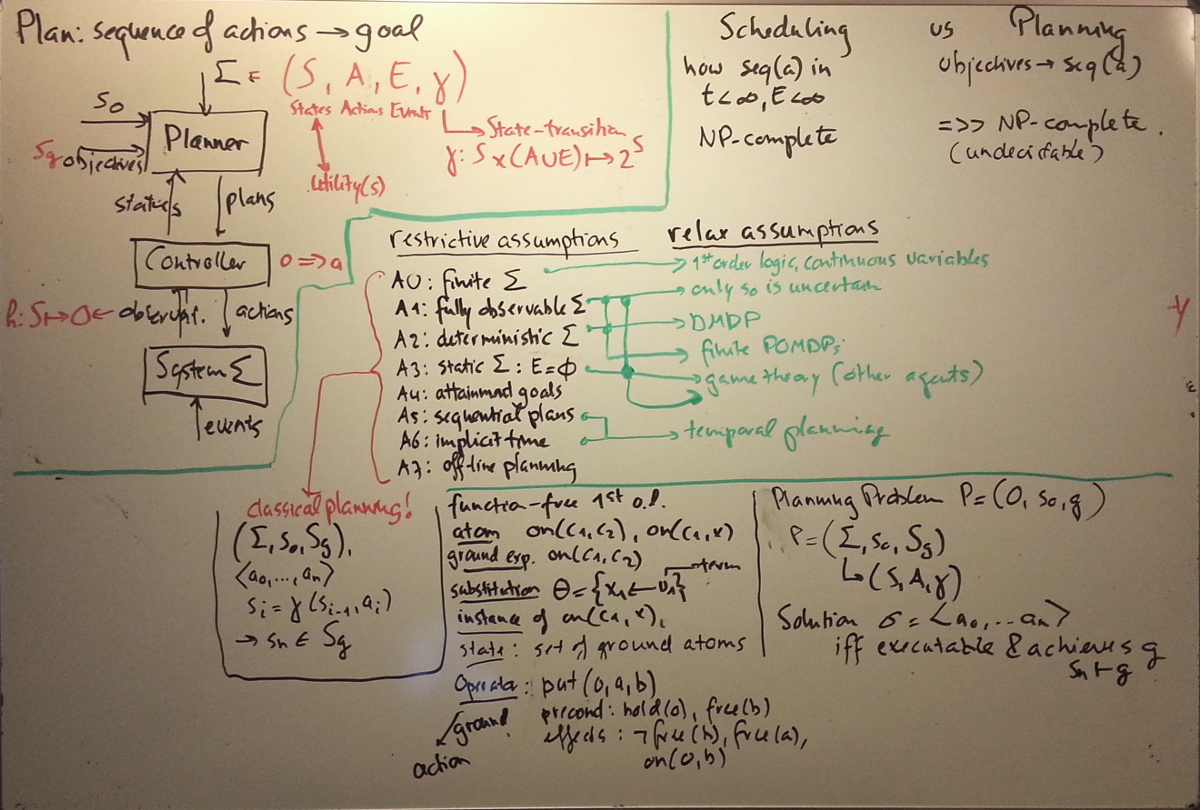
\includegraphics[width=180mm]{img/1.jpg}
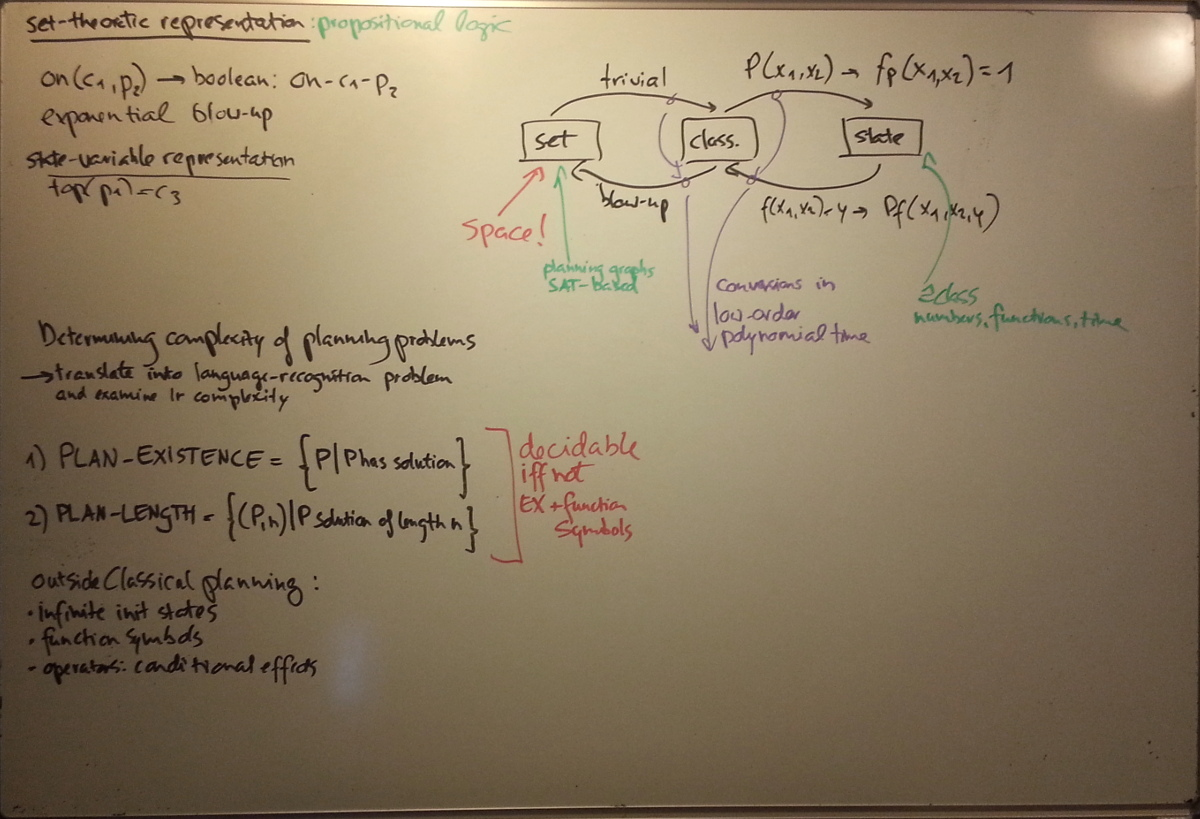
\includegraphics[width=180mm]{img/2.jpg}
\caption{..}
\label{ideas}
\end{figure}
\begin{figure}[ht!]
\centering
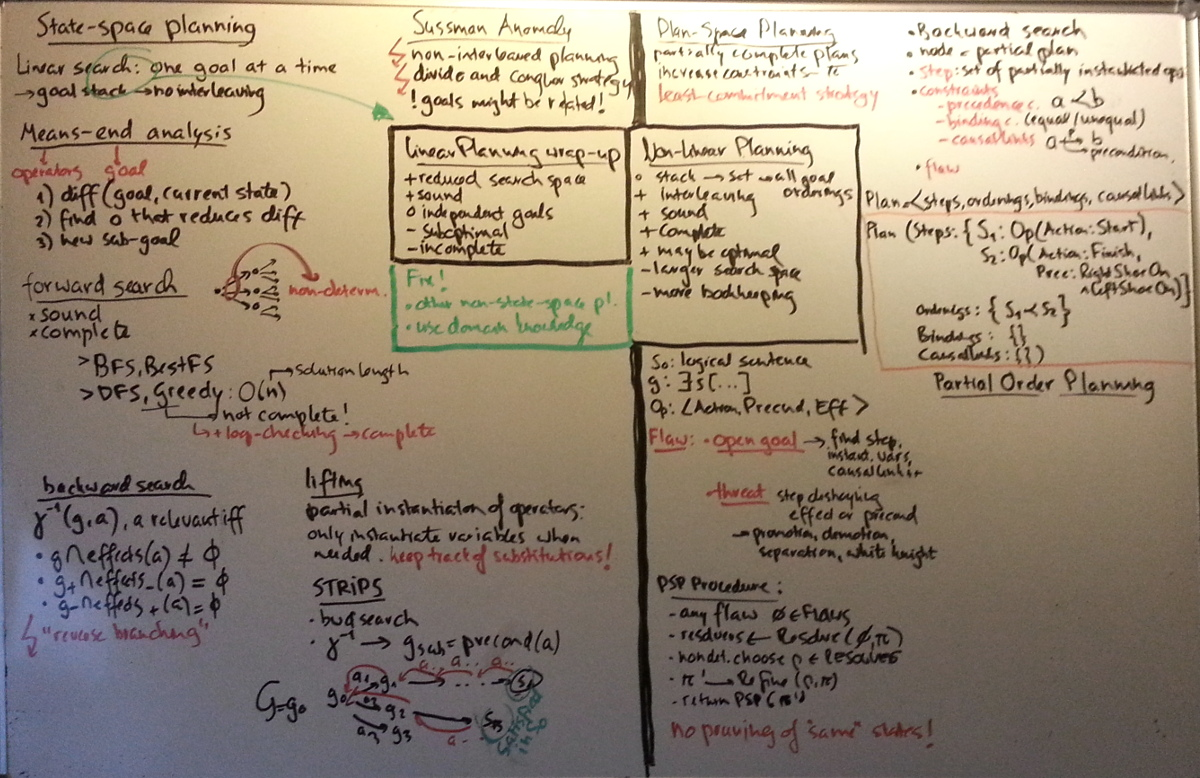
\includegraphics[width=180mm]{img/3.jpg}
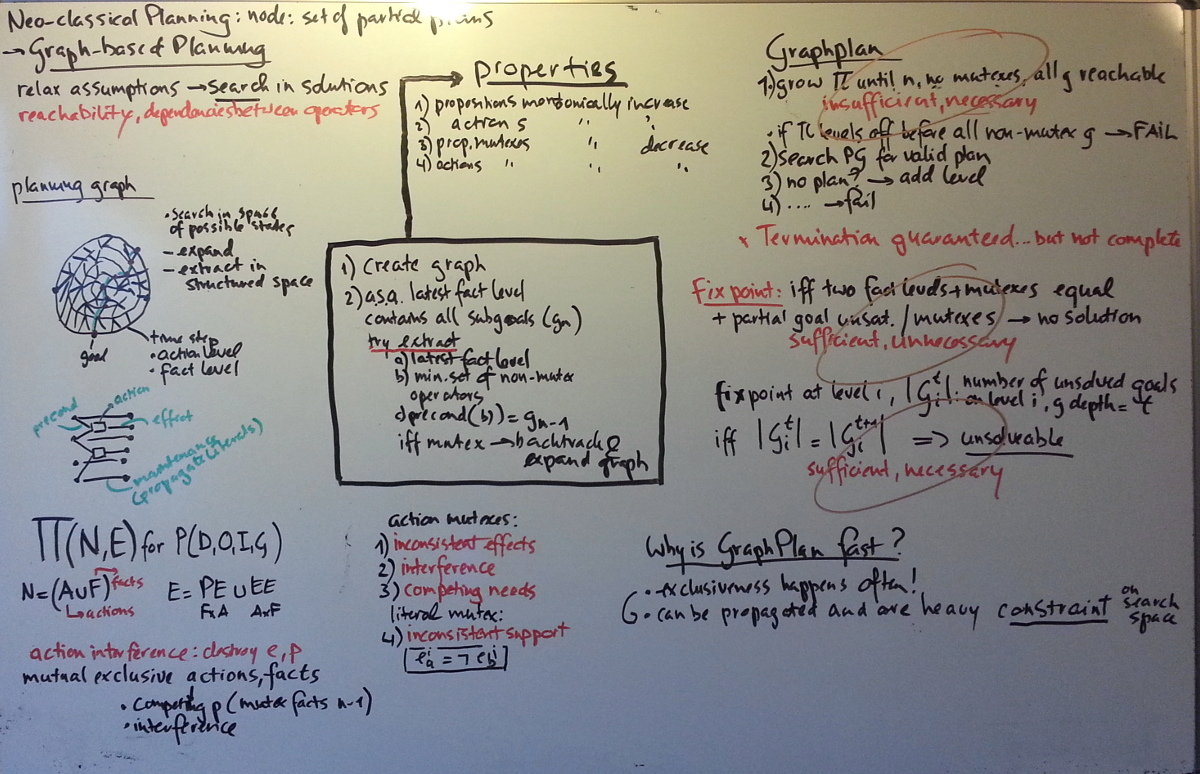
\includegraphics[width=180mm]{img/4.jpg}
\caption{..}
\label{ideas}
\end{figure}
\end{document}